\documentclass[../main.tex]{subfiles}
\graphicspath{{\subfix{images/}}}

\begin{document}

Dans cette section, vous allez expliquer les différents algorithmes qui vous paraissent importants pour votre projet. (Pour l'explication : son principe, les grandes lignes de comment il s'exécute, sa complexité,...)

\subsection{Programmation orientee objet}
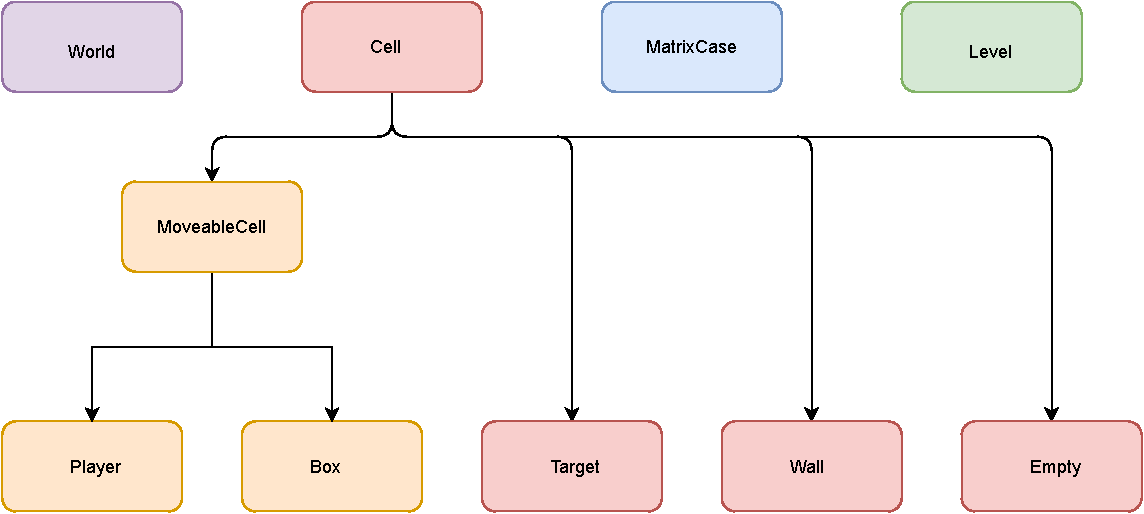
\includegraphics[width=1\textwidth,clip]{images/objects.pdf}

\subsection{Representation d'une map}
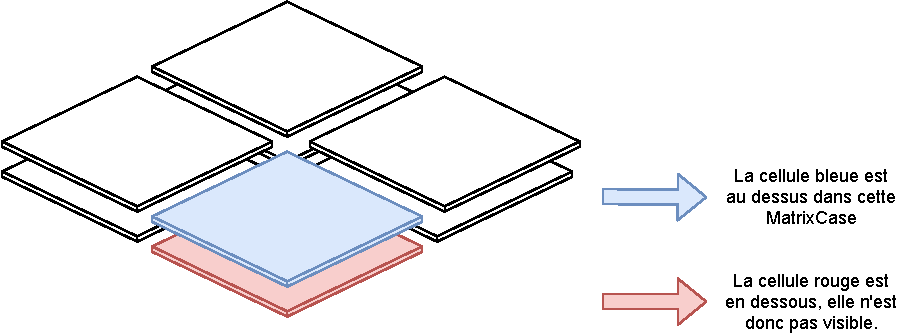
\includegraphics[width=1\textwidth,clip]{images/matrixCase.pdf}

\subsection{Chargement d'un niveau}

\subsection{Déplacements}

\subsection{Options utilisateur}

\subsection{Pack de textures}

\subsection{Génération aléatoire de niveau}
\subsubsection{Placement aléatoire}
\subsubsection{Backward induction}
\subsubsection{A* path finding}

\end{document}
